\documentclass[12pt,a4paper]{article}
\usepackage[utf8]{inputenc}
\usepackage[T1]{fontenc}
\usepackage[lithuanian]{babel}
\usepackage{graphicx}
\usepackage{caption}
\usepackage{float}
\usepackage{amsmath}
\usepackage{booktabs}
\usepackage{geometry}
\geometry{margin=2.5cm}

\title{Daugiasluoksnio perceptrono klasifikavimo užduotis naudojant KNIME}
\author{Vardas Pavardė}
\date{Vilnius, 2025}

\begin{document}
\maketitle
\begin{abstract}
Šiame darbe nagrinėjamas daugiasluoksnio perceptrono taikymas klasifikavimo užduočiai, naudojant KNIME platformą. 
Pateikiama duomenų analizė, paruošimas, modelio apmokymas, testavimas, hiperparametrų optimizavimas bei rezultatų vizualizacija. 
Taip pat lyginami perceptrono rezultatai su kitais mašininio mokymosi metodais.
\end{abstract}
\section{Duomenų analizė}
Naudoti duomenys: iris.csv iš UCI saugyklos.\newline
\textbf{Mokymui}: 120 įrašų (po 40 kiekvienai klasei).\\
\textbf{Testavimui}: 30 įrašų (po 10 kiekvienai klasei).

\section{Duomenų paruošimas KNIME sistemoje}
\begin{figure}[H]
    \centering
    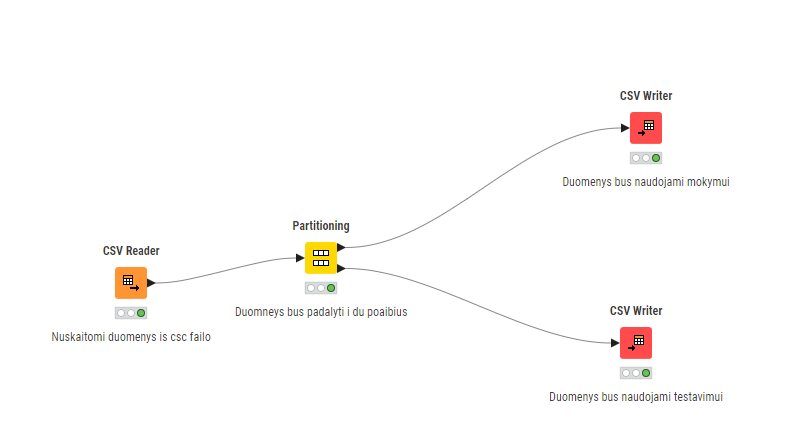
\includegraphics[width=0.9\textwidth]{KNIME_2.png}
    \caption{Užduočių seka, sudaranti duomenis mokymui ir testavimui}
\end{figure}
Trumpas aprašymas, kaip buvo atliktas padalijimas: naudota stratified sampling, Absolute 120.

\section{Daugiasluoksnio perceptrono apmokymas}
\begin{figure}[H]
    \centering
    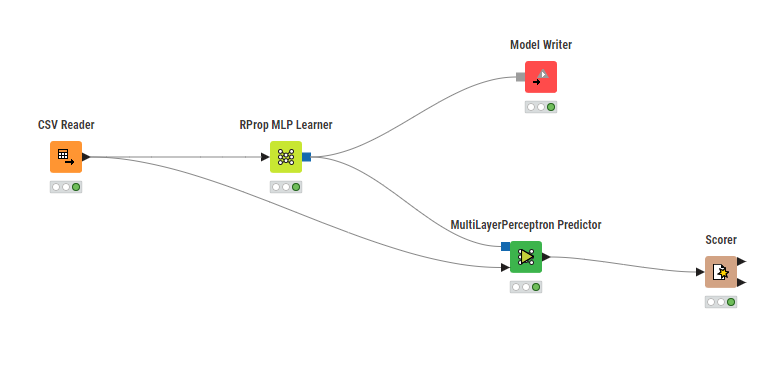
\includegraphics[width=0.9\textwidth]{KNIME_3.png}
    \caption{2 pav. Užduočių seka daugiasluoksniam perceptronui mokyti ir modeliui išsaugoti}
\end{figure}
Trumpas aprašymas: naudotas RProp MLP Learner, modelis išsaugotas su Model Writer.\\
Scorer komponentėje First Column: \texttt{class}, Second Column: \texttt{Prediction (class)}.\\
\textbf{Mokymo rezultatai}:
\begin{itemize}
    \item Klasifikavimo matrica: \textit{čia įdėkite matricą}
    \item Tikslumo metrikos: \textit{čia įrašyti metrikas}
    \item Klaidos kitimo grafikas:
    \begin{figure}[H]
        \centering
        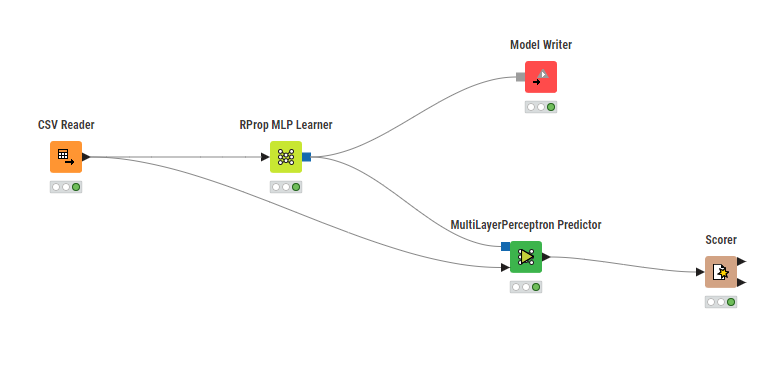
\includegraphics[width=0.9\textwidth]{KNIME_3.png}
        \caption{Paklaidos kitimas mokymo metu}
    \end{figure}
\end{itemize}

\section{Modelio testavimas}
\begin{figure}[H]
    \centering
    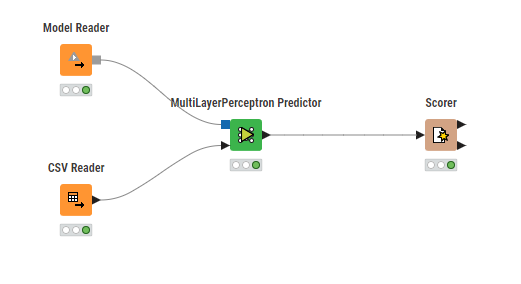
\includegraphics[width=0.9\textwidth]{KNIME_4.png}
    \caption{3 pav. Užduočių seka daugiasluoksniam perceptronui testuoti}
\end{figure}
\textbf{Testavimo rezultatai}:
\begin{itemize}
    \item Klasifikavimo matrica: \textit{čia įdėkite matricą}
    \item Tikslumo metrikos: \textit{čia įrašyti metrikas}
\end{itemize}

\section{Hiperparametrų optimizavimas}
\begin{figure}[H]
    \centering
    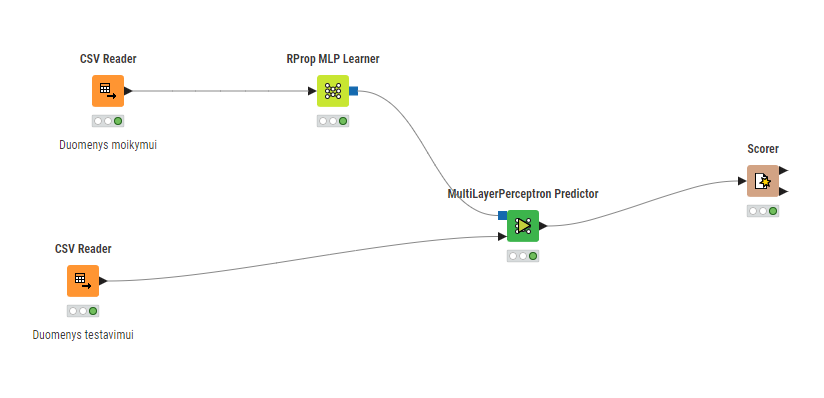
\includegraphics[width=0.9\textwidth]{KNIME_5.png}
    \caption{4 pav. Užduočių seka daugiasluoksniam perceptronui mokyti ir testuoti}
\end{figure}
Bandyti hiperparametrų rinkiniai:
\begin{itemize}
    \item Rinkinys 1: \texttt{Hidden layers: 1, Learning rate: 0.1, Epochs: 100}
    \item Rinkinys 2: ...
\end{itemize}
\textbf{Optimalūs hiperparametrai}: \textit{čia įrašyti rezultatus}

\section{Tikimybių, priskirtų klasių ir duomenų vizualizacija}
Norint pamatyti tikimybes ir priskirtą klasę visiems testavimo duomenims, naudotasi 4 paveiksle pavaizduota seka.

\begin{figure}[H]
    \centering
    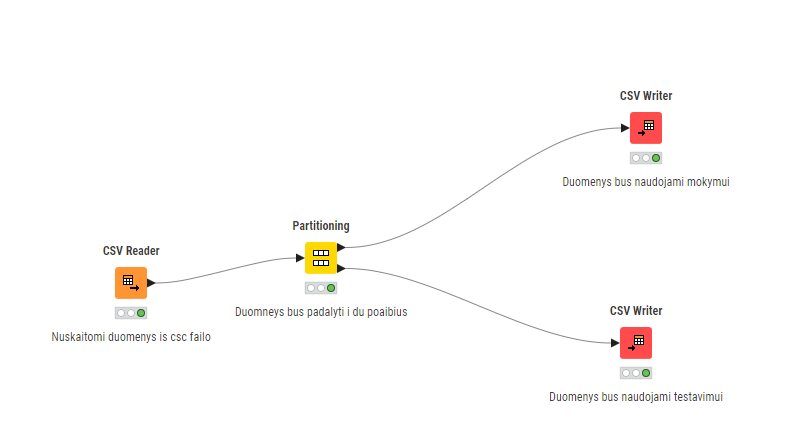
\includegraphics[width=0.9\textwidth]{KNIME_2.png}
    \caption{KNIME kodo blokas, naudojamas tikimybių ir klasės prognozių gavimui}
\end{figure}

\begin{table}[H]
    \centering
    \caption{Tikimybės ir klasės testavimo rinkinyje}
    \begin{tabular}{l l l l l l}
        \toprule
        Požymis 1 & ... & Tikra klasė & Tikimybė 1 & Tikimybė 2 & Priskirta klasė \\
        \midrule
        ... & ... & ... & ... & ... & ... \\
        \bottomrule
    \end{tabular}
\end{table}

Norint duomenis pavaizduoti XY koordinačių sistemoje, 4 paveiksle pateiktą seką papildėme komponentėmis Color Manager ir Scatter Plot Matrix.

\begin{figure}[H]
    \centering
    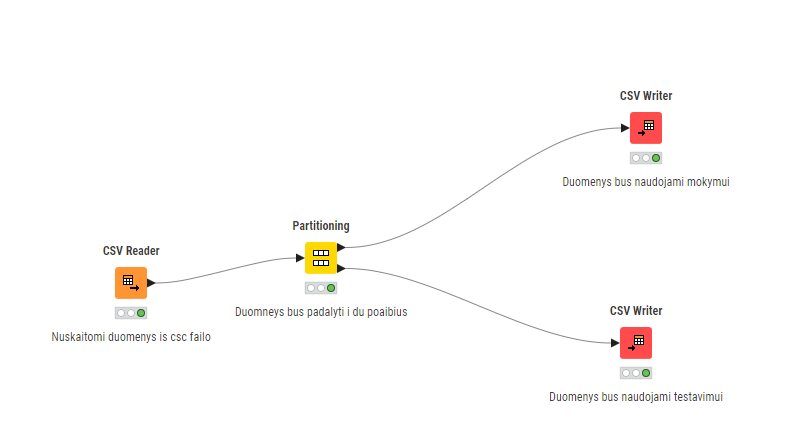
\includegraphics[width=0.9\textwidth]{KNIME_2.png}
    \caption{Mokymo duomenys XY koordinačių sistemoje}
\end{figure}

\begin{figure}[H]
    \centering
    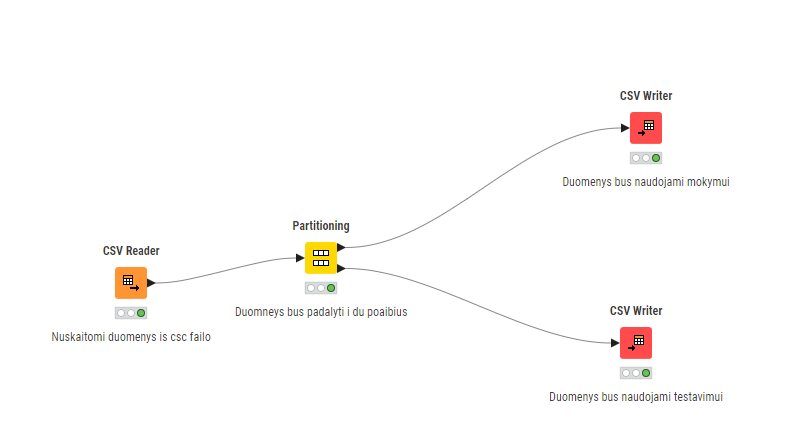
\includegraphics[width=0.9\textwidth]{KNIME_2.png}
    \caption{Testavimo duomenys XY koordinačių sistemoje}
\end{figure}

\begin{figure}[H]
    \centering
    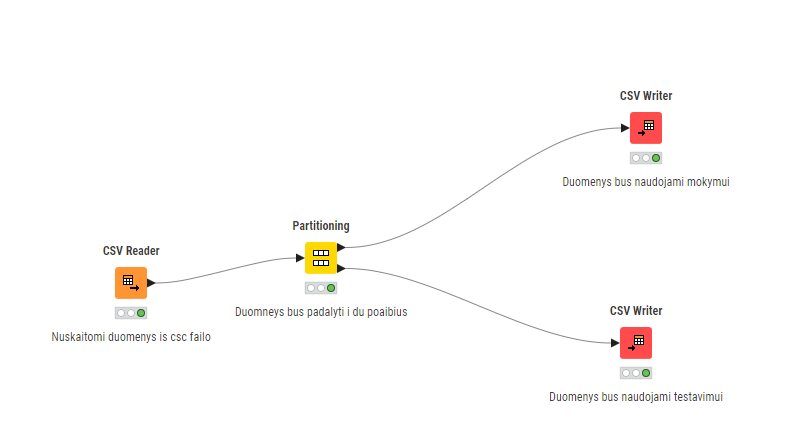
\includegraphics[width=0.9\textwidth]{KNIME_2.png}
    \caption{KNIME kodo blokas XY duomenų vizualizavimui (Color Manager ir Scatter Plot Matrix)}
\end{figure}

\section{Daugiasluoksnio perceptrono palyginimas su kitais mašininio mokymosi metodais}
Papildomai naudoti metodai:
\begin{itemize}
    \item \textbf{Statistics} (Naudotas KNIME komponentas)
    \item \textbf{Decision Tree Learner} – rezultatai palyginti su perceptrono rezultatais
\end{itemize}

\begin{figure}[H]
    \centering
    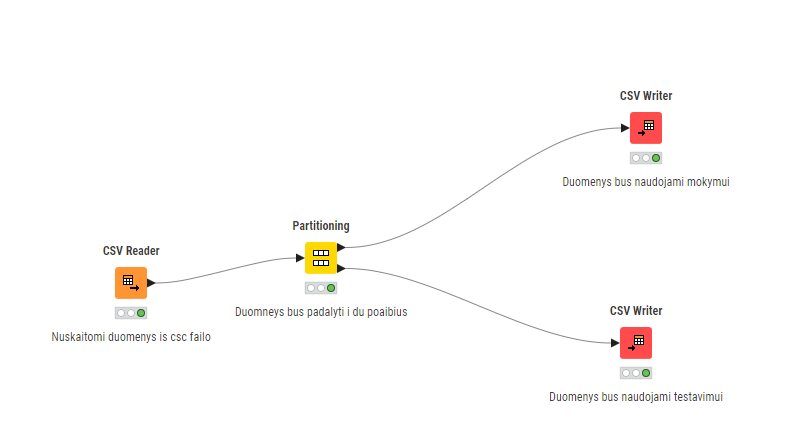
\includegraphics[width=0.9\textwidth]{KNIME_2.png}
    \caption{Statistics metodo taikymo seka KNIME}
\end{figure}

\begin{figure}[H]
    \centering
    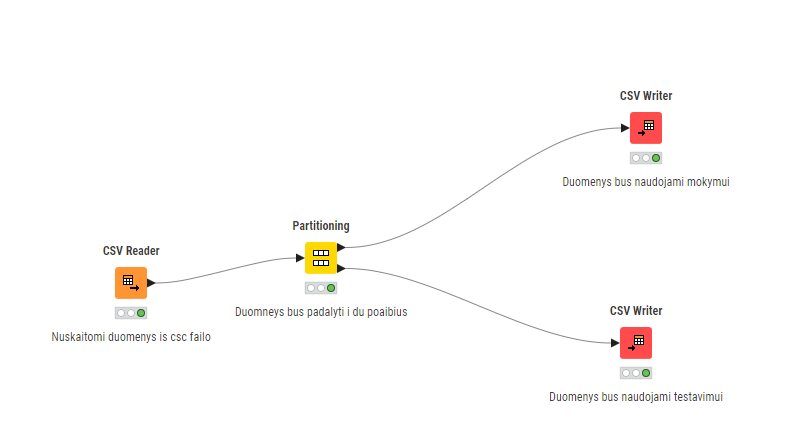
\includegraphics[width=0.9\textwidth]{KNIME_2.png}
    \caption{Decision Tree metodo taikymo seka KNIME}
\end{figure}

\begin{figure}[H]
    \centering
    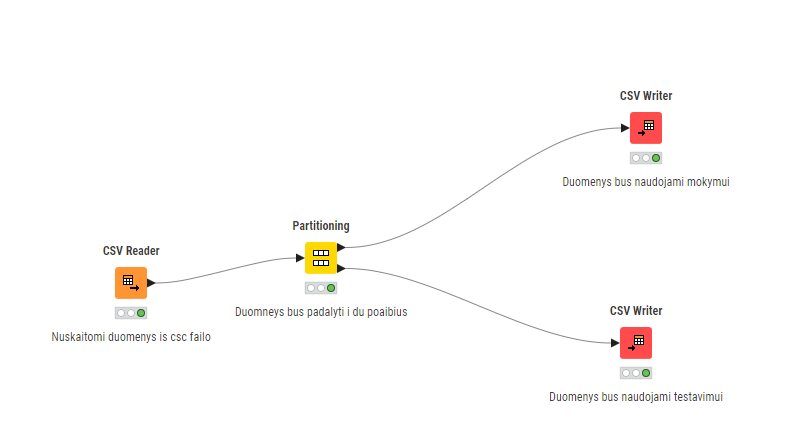
\includegraphics[width=0.9\textwidth]{KNIME_2.png}
    \caption{Decision Tree schema ir rezultatai}
\end{figure}

Palyginimo santrauka: tikslumai, interpretacija, komentarai apie skirtumus.

\end{document}